\documentclass{article}

\usepackage{enumitem}
\usepackage{listings}
\usepackage{color}
\usepackage{amsmath}
\usepackage{hyperref}
\usepackage{graphicx}
\usepackage{pgffor}
\usepackage{xparse}
\usepackage{expl3}
\usepackage{tabularx, makecell}
\usepackage{multirow}
% \usepackage{booktabs}
\usepackage{indentfirst}
\usepackage{lipsum}
\usepackage{sectsty}
\usepackage[utf8]{inputenc}
% \usepackage{csquotes}
% \usepackage{xcolor}
% \usepackage{fancyvrb}
% \usepackage{fancyhdr}
% \usepackage{fancyvrb}
% \usepackage[most]{tcolorbox}
% \usepackage{blindtext}
\usepackage{caption}
% \usepackage{etoolbox}
\usepackage{mdframed}
\usepackage[nomessages]{fp}
% \usepackage{pgfplots}
\usepackage{geometry}

\graphicspath{{./}}

\definecolor{codegreen}{rgb}{0,0.6,0}
\definecolor{codegray}{rgb}{0.5,0.5,0.5}
\definecolor{codepurple}{rgb}{0.58,0,0.82}
\definecolor{backcolour}{rgb}{0.95,0.95,0.92}

\sectionfont{\bfseries\Large\center} 

% Lstlisting configuartions for C++
\lstset{
	language=C++,
	frame=single,
	rulecolor=\color{gray},
	basicstyle=\fontsize{5}{5}\ttfamily,
	keywordstyle=\color{blue},
	stringstyle=\color{orange},
	commentstyle=\color{gray},
	extendedchars=true,
	keepspaces=true,
	numbers=left,
	numbersep=5pt,
	numberstyle=\color{gray},
	tabsize=4,
	morecomment=[l][\color{gray}]{\#}
}

% Lstlisting configuartions for algorithm code
\newcounter{nalg}[section]
\renewcommand{\thenalg}{\arabic{nalg}}
\DeclareCaptionLabelFormat{algocaption}{\textbf{Algorithm \thenalg}}
\lstnewenvironment{algorithm}[1][]
{
    \refstepcounter{nalg}
    \captionsetup{labelformat=algocaption,labelsep=colon}
    \lstset{
        mathescape=true,
        frame=tB,
        numbers=left, 
        numberstyle=\tiny,
        basicstyle=\scriptsize, 
        keywordstyle=\color{blue}\bfseries\em,
        keywords={,input, output, return, datatype, function, in, if, else, foreach, while, begin, end, then, }
        numbers=left,
        xleftmargin=.04\textwidth,
        #1
    }
}{}

\begin{document}
	%Custom commands
	% <Square cases>
		\makeatletter
		\newenvironment{sqcases} {
			\matrix@check\sqcases\env@sqcases
		}{
			\endarray \right.
		}
		\def\env@sqcases {
			\let \@ifnextchar \new@ifnextchar
			\left \lbrack
			\def \arraystretch{1.2}
			\array{@{}l@{\quad}l@{}}
		}
		\makeatother
	% </Square cases>

	% Html like line
		\newcommand\hr{\par\vspace{-.5\ht\strutbox}\noindent\hrulefill\par}

	%Begin of the document

	\title{MMC Laboratory work\_2}
	\author{Terman Emil FAF161}
	\maketitle
	
	\begin{center}
	
\includegraphics{imgs/UTM_logo.png}
	\end{center}
	\begin{flushright}
		Prof: V. Bostan
	\end{flushright}
	\begin{center}
	\LaTeX
	\end{center}
	\pagebreak %------------------------------------------------------------------End of title page
	
	\section{Root finding}
		\begin{center}
			\par Find the root of the function
			\[
				f(x) = \sqrt{x} - e^{-x}
			\]
			using Bisection, Newton, Simplified Newton and Secant methods.
			\hr
		\end{center}

		In these graphs is shown how fast a method converges to the solution.
		\begin{center} \begin{figure}[!ht]
			\begin{mdframed} \begin{center}
				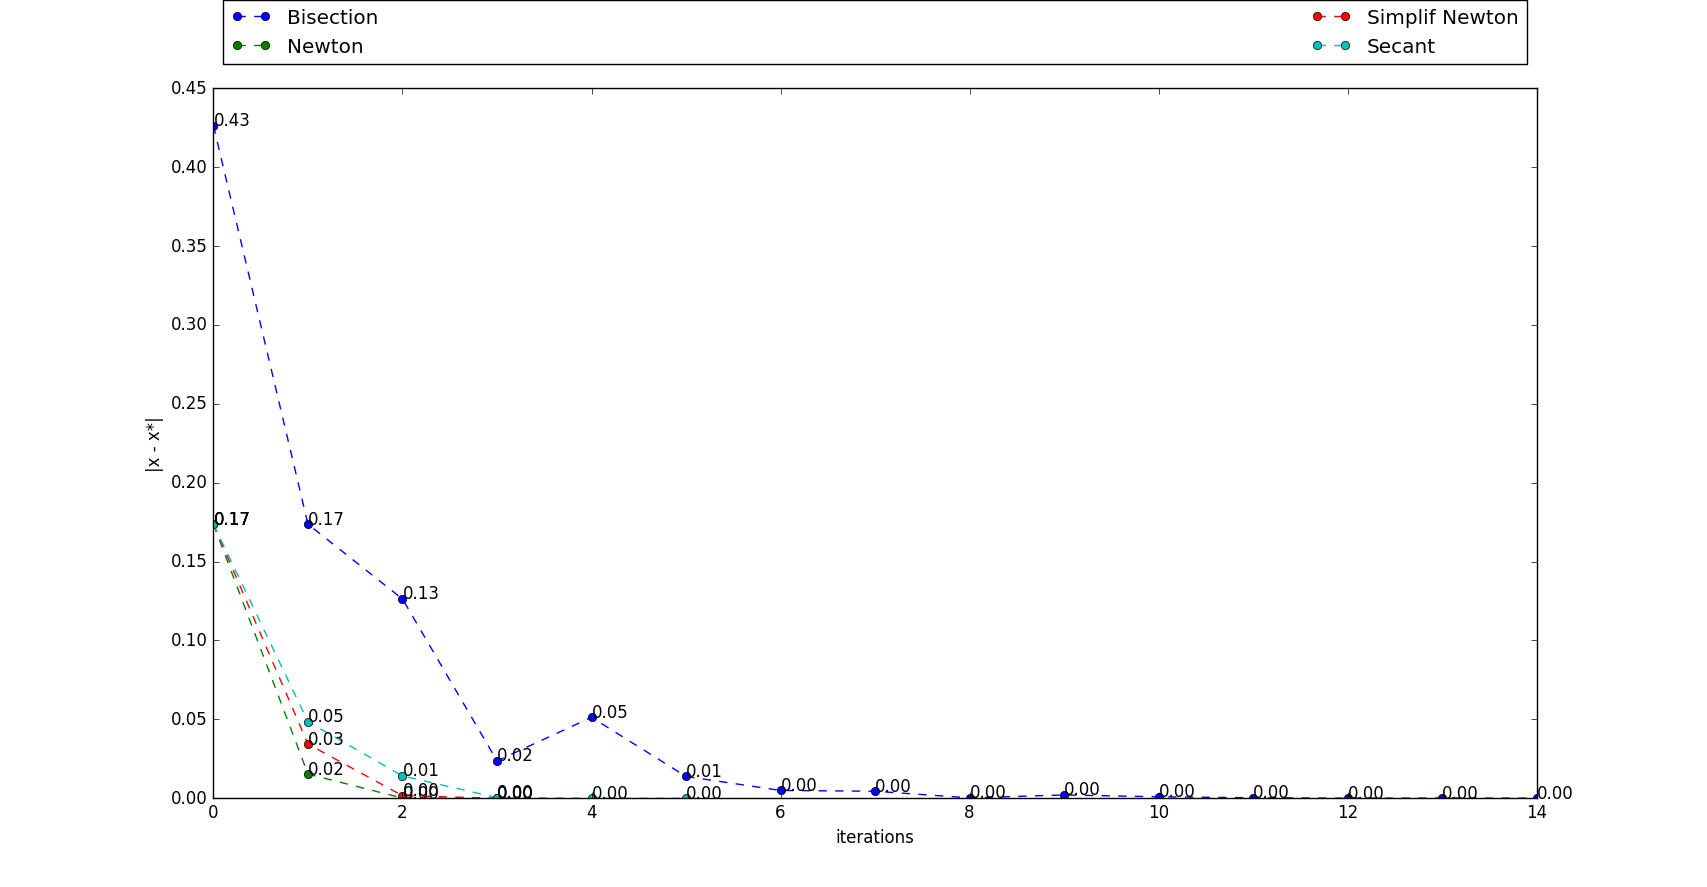
\includegraphics[scale=0.37]{./imgs/Ex1Plot.png}
				\caption{Convergence graph.}
			\end{center} \end{mdframed}
			\label{fig:graph1}
		\end{figure} \end{center}

		\begin{center} \begin{figure}[!ht]
			\begin{mdframed} \begin{center}
				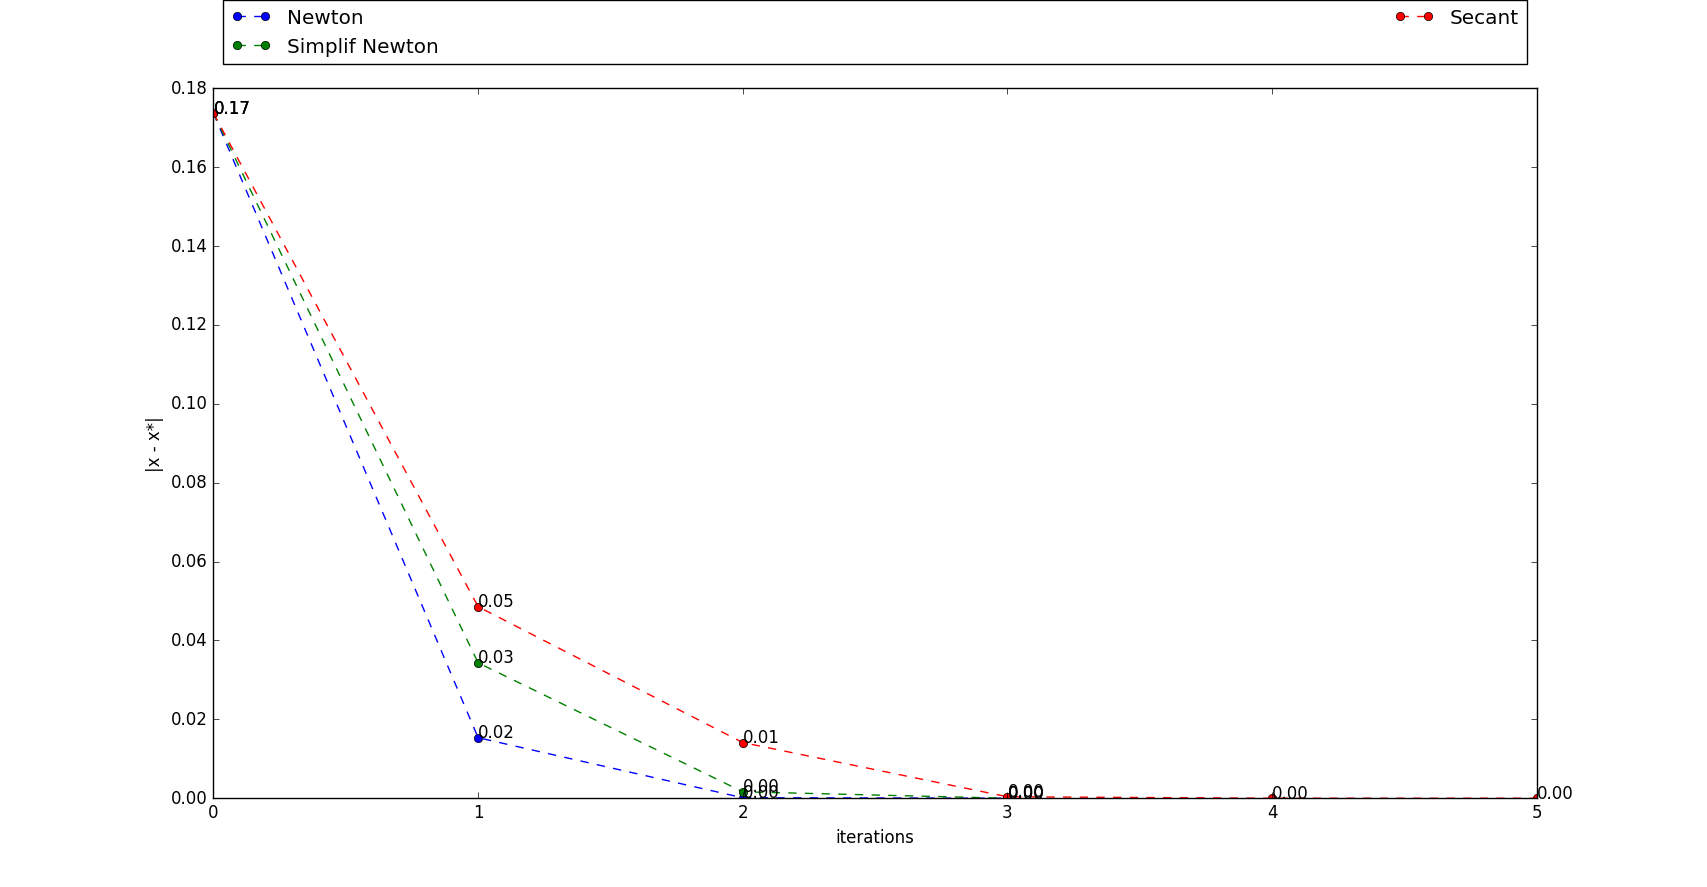
\includegraphics[scale=0.38]{./imgs/Ex1Plot2.png}
				\caption{Convergence graph (Without Bisection).}
			\end{center} \end{mdframed}
			\label{fig:graph2}
		\end{figure} \end{center}

		\begin{center} \begin{tabular}{|c|c|c|c|c|}
			\hline
			$i$ & Bisection & Newton & S. Newton & Secant\\
			\hline
			1 & 0.43000 & 0.01535 & 0.17369 & 0.04856\\ 
			\hline
			2 & 0.17369 & 0.00012 & 0.03433 & 0.01411\\
			\hline
			3 & 0.12630 & 0.00000 & 0.00163 & 0.00037\\
			\hline
			4 & 0.02369 & 0.00000 & 0.00000 & 0.00000\\
			\hline
			5 & 0.05130 & - & - & 0.00000\\
			\hline
			6 & 0.01380 & - & - & -\\
			% \hline
			\multicolumn{5}{c}{...}\\
			% \hline
			14 & 0.00004 & - & - & -\\
			\hline
		\end{tabular} \end{center}

		\begin{enumerate}
			\item \textbf{Newton}
				\begin{itemize}
					\item We can clearly see that \textit{Newton} method is the fastest to converge. But we should also note that it's the most complicated method, since derivation is required.

					\item Also, an initial guess is required: if there is a horizontal tangent line at $x_0$, then the derivation is 0 and we can't have divisions by 0.

					\item If the function has 2 roots, we must provide an initial guess near the solution we want, otherwise, we will recive the wrong root.
				\end{itemize}
			\item \textbf{Bisection}
				\begin{itemize}
					\item \textit{Bisection} method is much slower, but simplier. Sometimes we don't need a better function.

					\item Also, the given interval $[a, b]$ must respect the following condition: 

					\[f(a) * f(b) < 0\]
					While with the Newton's method we can try a wild guess, for example $x_0 = 100$ while the root is 1, we would still get the right result, but with the \textit{Bisection} method, we need to provide a big enough interval in which the root is sure to be found.
				\end{itemize}
			\item \textbf{Simplified Newton} isn't much behind Newton's method. It converges slightly slower but it doesn't require derivation.
			\[
				x_{i + 1} = x_i - \frac{f^2(x_i)}{f(x_i + f(x_i)) - f(x_i)}
			\]
			\item \textbf{Secant} method requires more iterations, but it can be faster in time than Newton's, since it doesn't require 2 function evaluation per iteration.
		\end{enumerate}

		\newpage
		\section{Order of operations}
			\par In this exercise is required to compute the root using the program from the previous exercise, for different forms of the same function and different ranges or guesses.
			\[
				f(x) = x^3 - 3x^2 + 3x - 1
			\]

			\begin{center} \begin{figure}[!ht]
				\begin{mdframed} \begin{center}
					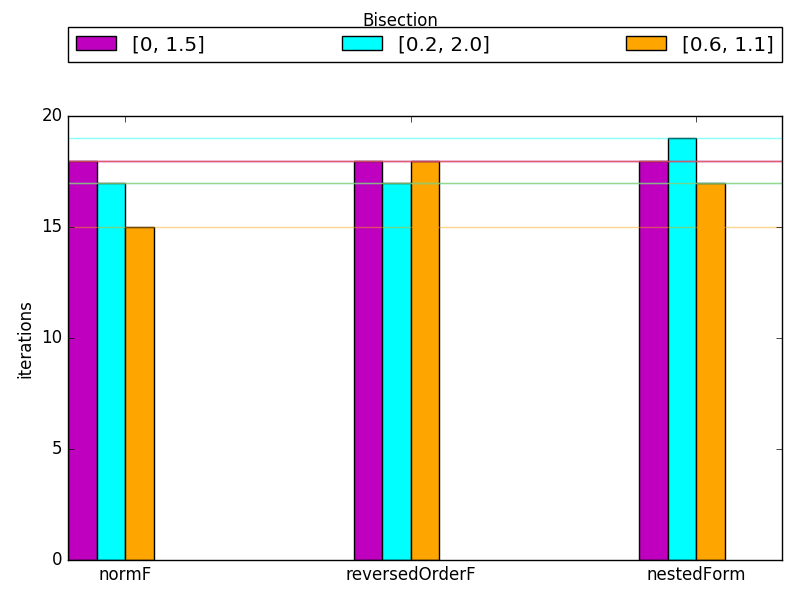
\includegraphics[scale=0.6]{./imgs/Ex2Bis.png}
					\caption{Bisection.}
				\end{center} \end{mdframed}
				\label{fig:barPlot1}
			\end{figure} \end{center}


			\begin{center} \begin{figure}[!ht]
				\begin{mdframed} \begin{center}
					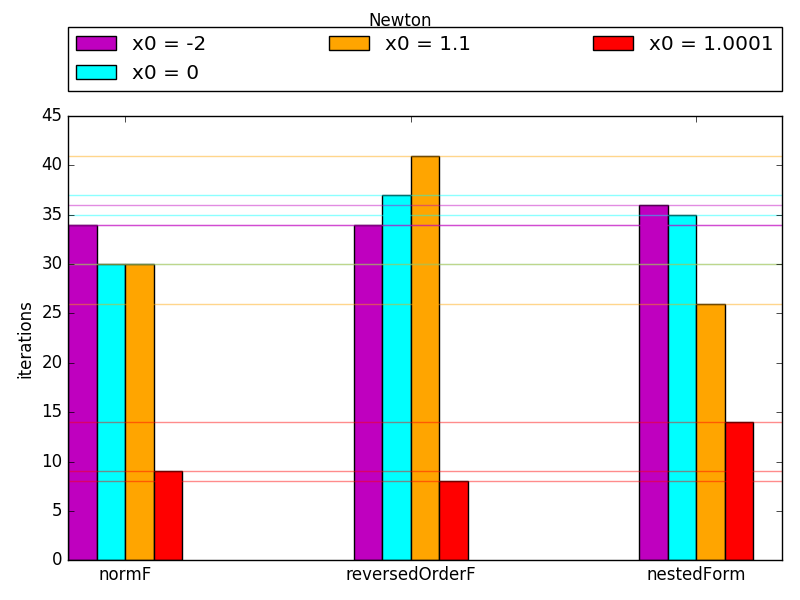
\includegraphics[scale=0.6]{./imgs/Ex2Nwt.png}
					\caption{Newton's.}
				\end{center} \end{mdframed}
				\label{fig:barPlot2}
			\end{figure} \end{center}

			\begin{center} \begin{figure}[!ht]
				\begin{mdframed} \begin{center}
					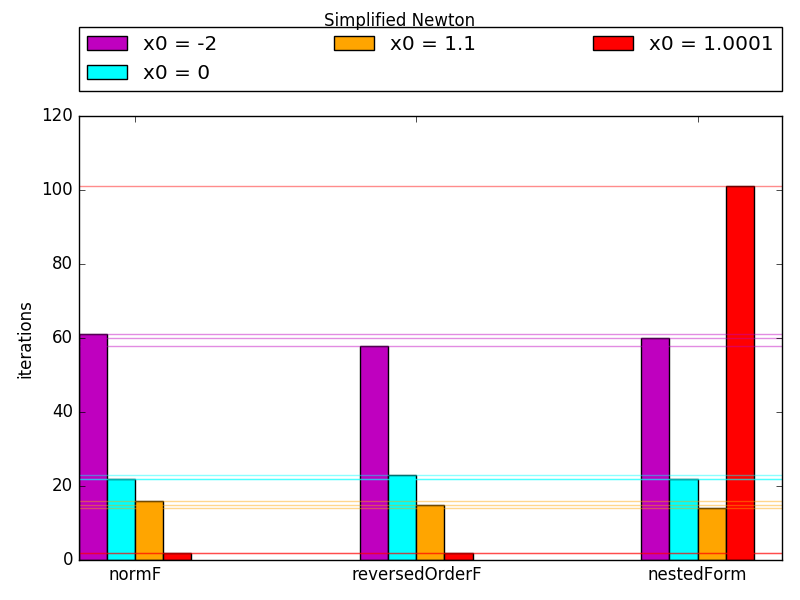
\includegraphics[scale=0.6]{./imgs/Ex2SNwt.png}
					\caption{Simplified Newton.}
				\end{center} \end{mdframed}
				\label{fig:barPlot3}
			\end{figure} \end{center}


			\begin{center} \begin{figure}[!ht]
				\begin{mdframed} \begin{center}
					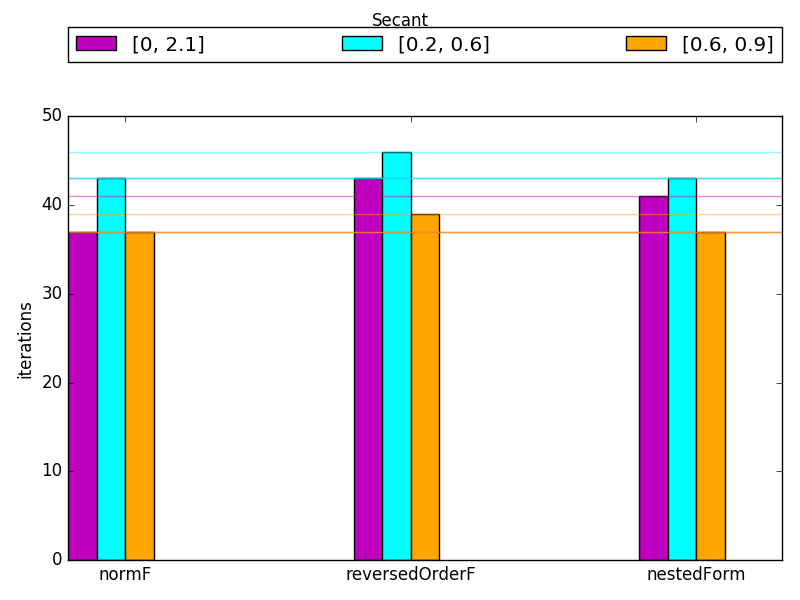
\includegraphics[scale=0.6]{./imgs/Ex2Sect.png}
					\caption{Secant.}
				\end{center} \end{mdframed}
				\label{fig:barPlot4}
			\end{figure} \end{center}

			\par Theoreticly, the normal and nested forms should compute the result in less iterations, because adding adding small to big numbers, minimizes the loss of significance error, producing less errors, therefore - less iterations. The nested form aproach also reduces the calculation errors. But in this case, no notable difference is observed.

			\newpage
			\section{Integrals?}
				\begin{center}
					For $c = 69.35935935935935958696$ (for example), \textbf{Newton}'s method doesn't converge.\\
					\begin{tabular}{|c|c|c|}
						\hline
						$i$ & x0 & x1\\
						\hline
						1 & 0.98578724978303855497 & 0.98558237769985945764\\
						\hline
						2 & 0.98558237769985945764 & 0.98558233511329373933\\
						\hline
						3 & 0.98558233511329373933 & 0.98558233511329\textbf{185195}\\
						\hline
						4 & 0.98558233511329\textbf{185195} & 0.98558233511329\textit{207399}\\
						\hline
						5 & 0.98558233511329\textit{207399} & 0.98558233511329\textbf{185195}\\
						\hline
						6 & 0.98558233511329\textbf{185195} & 0.98558233511329\textit{207399}\\
						\hline
						7 & 0.98558233511329\textit{207399} & 0.98558233511329\textbf{185195}\\
						\hline
						8 & 0.98558233511329\textbf{185195} & 0.98558233511329\textit{207399}\\
						\hline
						9 & 0.98558233511329\textit{207399} & 0.98558233511329\textbf{185195}\\
						\multicolumn{3}{c}{...}
					\end{tabular}
				\end{center}
				\par Here we have an oscilation between 2 values, because of the roundoff float precision.
\end{document}
